% l = 8
% \mbox{}\\[-0.75in]
\begin{figure}[!b]
\begin{center}
\subfloat{
\resizebox{8cm}{4.5cm}{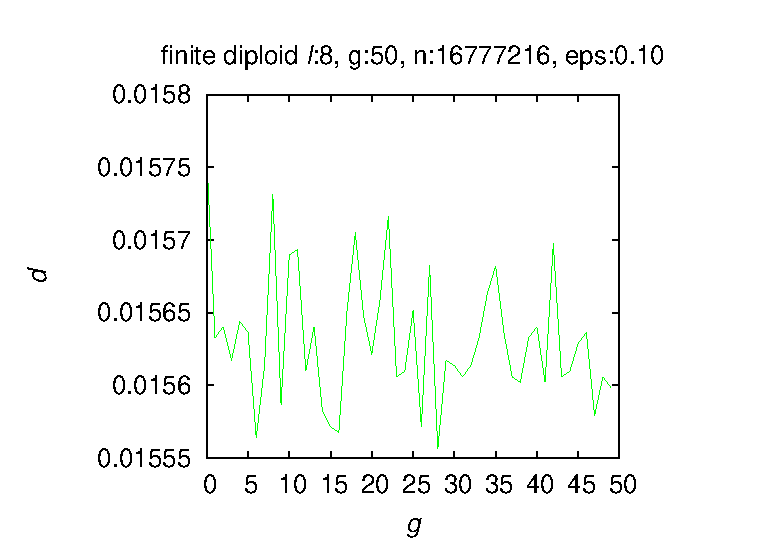
\includegraphics{figures/eps/vio/mu/b8/e0.1/n00004096_fin_dip.eps}}}\hspace{-3em}%
\subfloat{
\resizebox{8cm}{4.5cm}{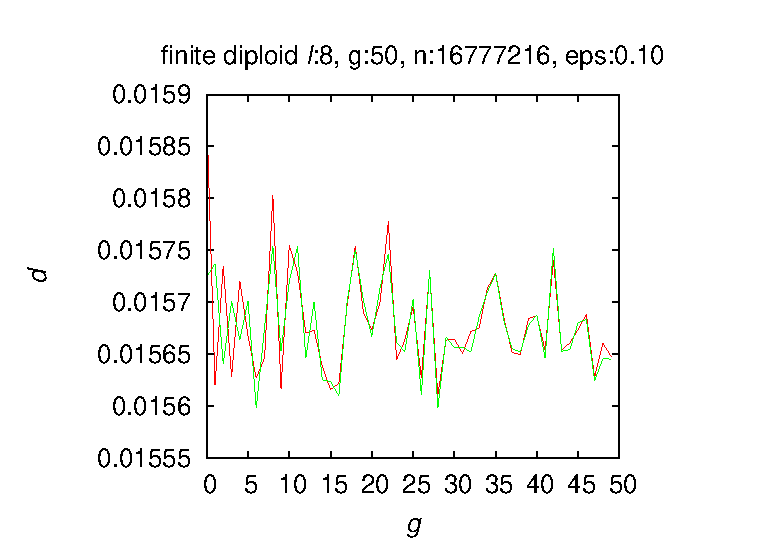
\includegraphics{figures/eps/vio/mu/b8/e0.1/n00004096_fin_dip_wovio.eps}}}\vspace{-1em}  \hspace{-3em}%
\end{center}
\begin{center}
\subfloat{
\resizebox{8cm}{4.5cm}{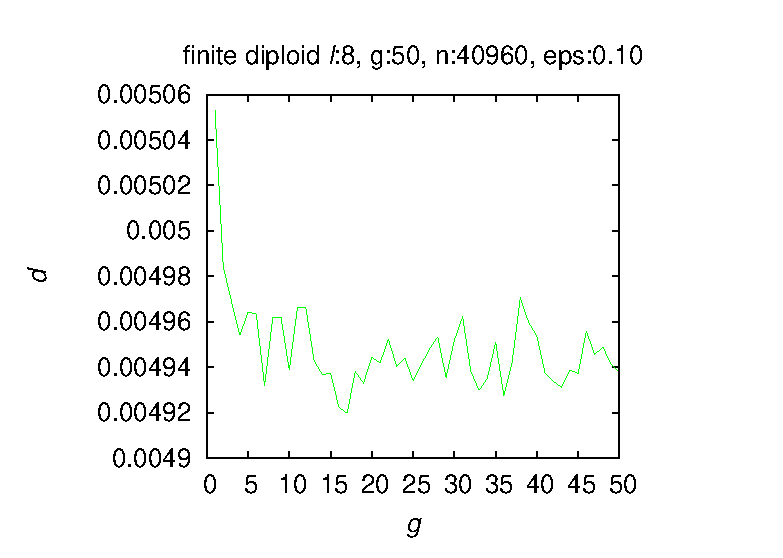
\includegraphics{figures/eps/vio/mu/b8/e0.1/n00040960_fin_dip.eps}}}\hspace{-3em}%
\subfloat{
\resizebox{8cm}{4.5cm}{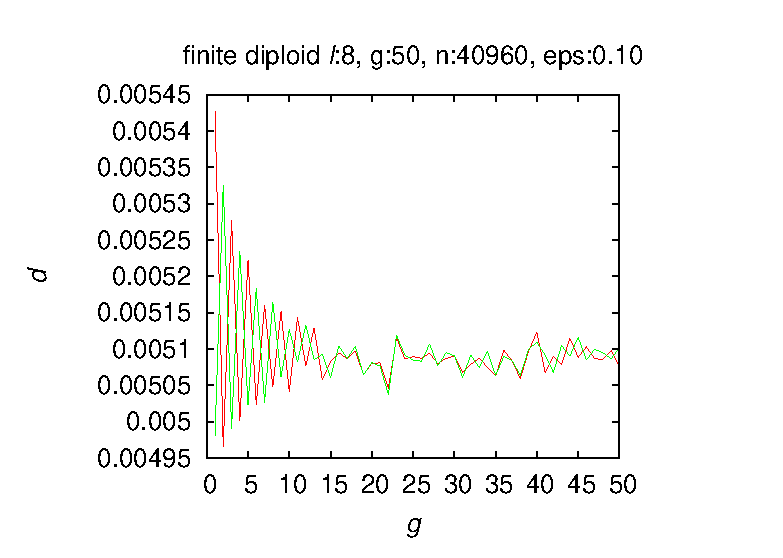
\includegraphics{figures/eps/vio/mu/b8/e0.1/n00040960_fin_dip_wovio.eps}}}\vspace{-1em}  \hspace{-3em}%
\end{center}

\begin{center}
\subfloat{
\resizebox{8cm}{4.5cm}{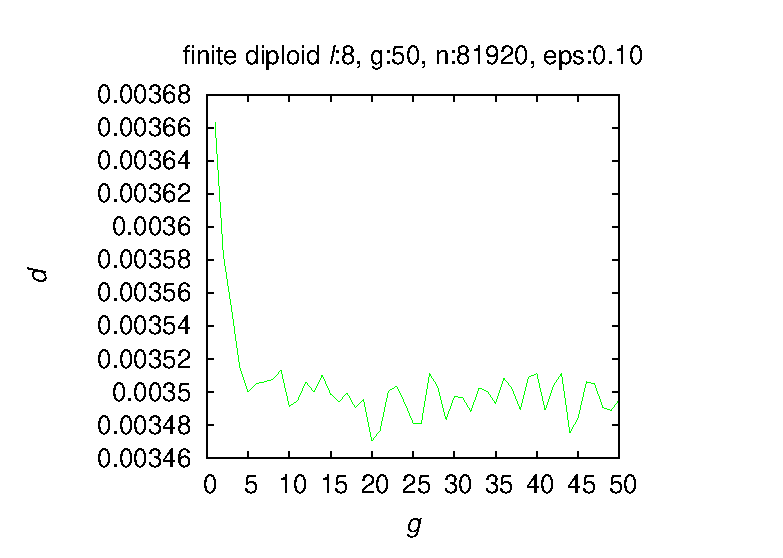
\includegraphics{figures/eps/vio/mu/b8/e0.1/n00081920_fin_dip.eps}}}\hspace{-3em}%
\subfloat{
\resizebox{8cm}{4.5cm}{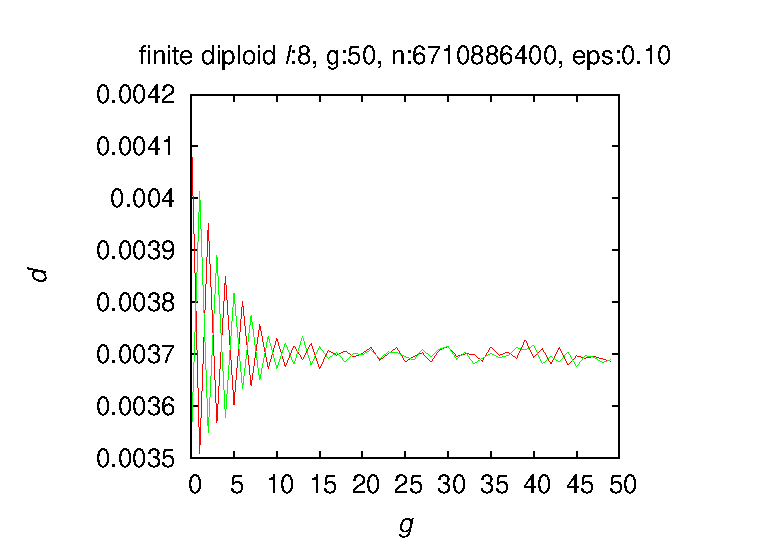
\includegraphics{figures/eps/vio/mu/b8/e0.1/n00081920_fin_dip_wovio.eps}}}\vspace{-1em}  \hspace{-3em}%
\end{center}

\begin{center}
\subfloat{
\resizebox{8cm}{4.5cm}{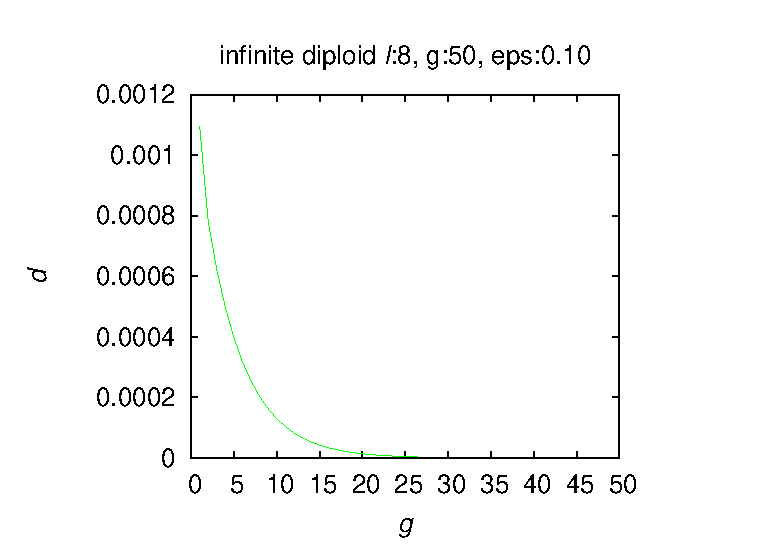
\includegraphics{figures/eps/vio/mu/b8/e0.1/inf_dip.eps}}}\hspace{-3em}%
\subfloat{
\resizebox{8cm}{4.5cm}{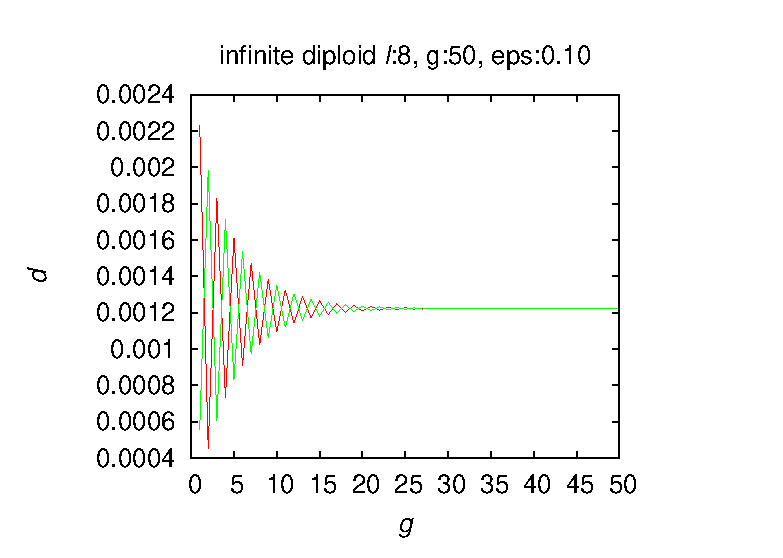
\includegraphics{figures/eps/vio/mu/b8/e0.1/inf_dip_wovio.eps}}}\vspace{-0.5em}  \hspace{-3em}%


\caption[\textbf{Infinite and finite diploid population behavior for $\bm{\mu}$ violation, $\ell = 8$ and $\bm{\epsilon} = 0.1$}]
{\textbf{Infinite and finite diploid population behavior for $\bm{\mu}$ violation, $\ell = 8$ and $\bm{\epsilon} = 0.1$:} 
  In left column, $d'$ is distance of finite or infinite population to limit $\bm{z}^\ast$ for $g$ generations. 
  In right column, $d$ is distance of finite or infinite population to limits $\bm{p}^\ast$ and $\bm{q}^\ast$. Green line is distance to $\bm{p*}$ and red line is distance to $\bm{q*}$.}
\label{oscillation_8d_vio_mu_0.1}
\end{center}
\end{figure}

% l = 10

\begin{figure}[h]
\begin{center}
\subfloat{
\resizebox{8cm}{4.5cm}{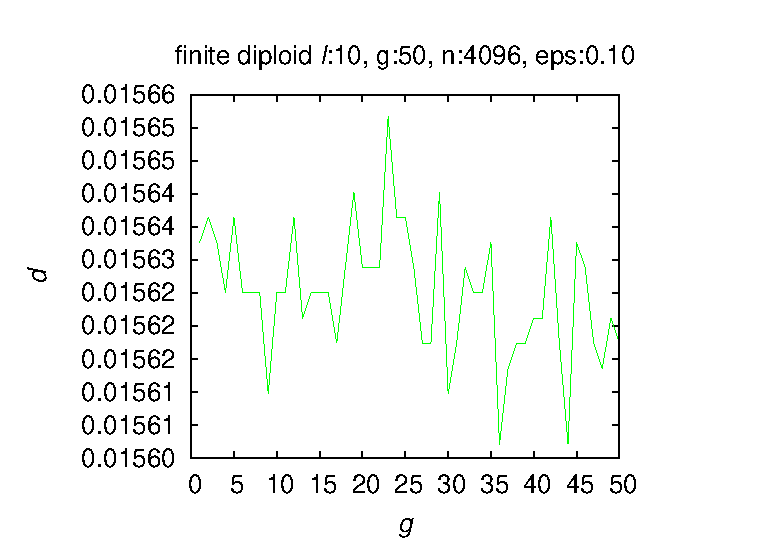
\includegraphics{figures/eps/vio/mu/b10/e0.1/n00004096_fin_dip.eps}}}\hspace{-3em}%
\subfloat{
\resizebox{8cm}{4.5cm}{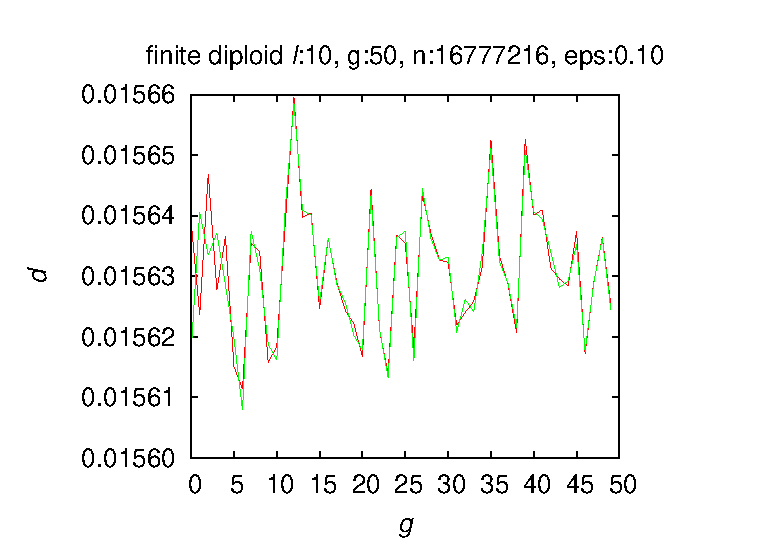
\includegraphics{figures/eps/vio/mu/b10/e0.1/n00004096_fin_dip_wovio.eps}}}\vspace{-1em}  \hspace{-3em}%
\end{center}
\begin{center}
\subfloat{
\resizebox{8cm}{4.5cm}{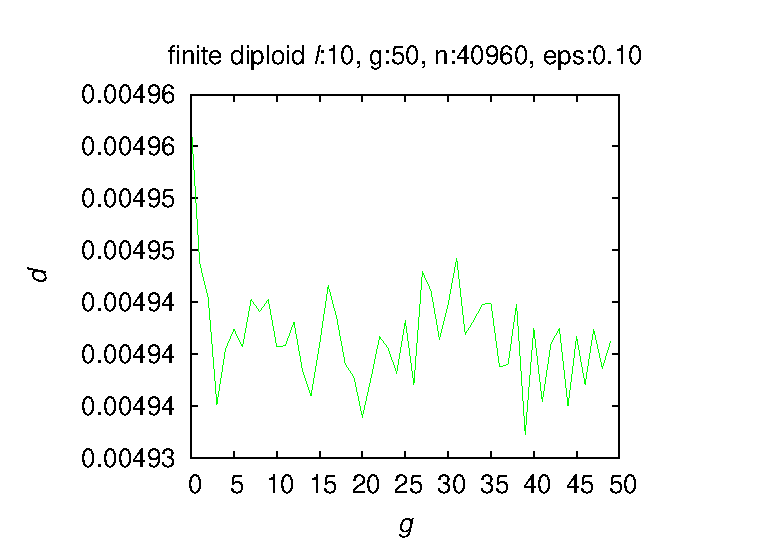
\includegraphics{figures/eps/vio/mu/b10/e0.1/n00040960_fin_dip.eps}}}\hspace{-3em}%
\subfloat{
\resizebox{8cm}{4.5cm}{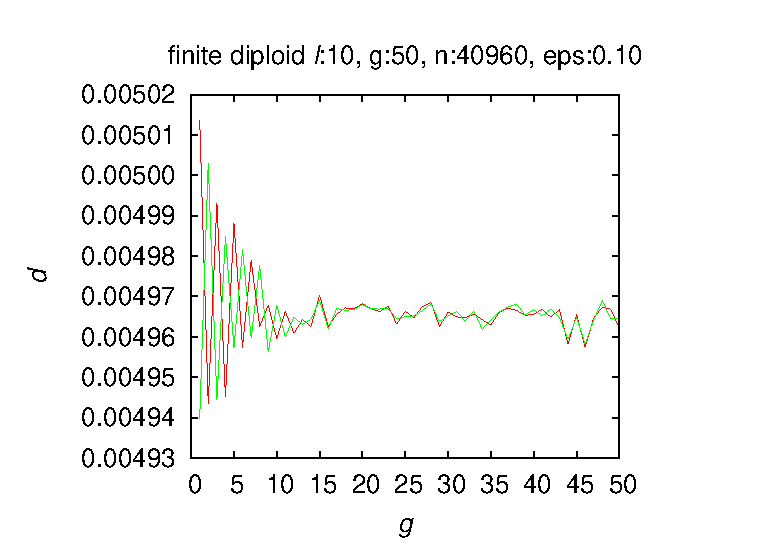
\includegraphics{figures/eps/vio/mu/b10/e0.1/n00040960_fin_dip_wovio.eps}}}\vspace{-1em}  \hspace{-3em}%
\end{center}


\begin{center}
\subfloat{
\resizebox{8cm}{4.5cm}{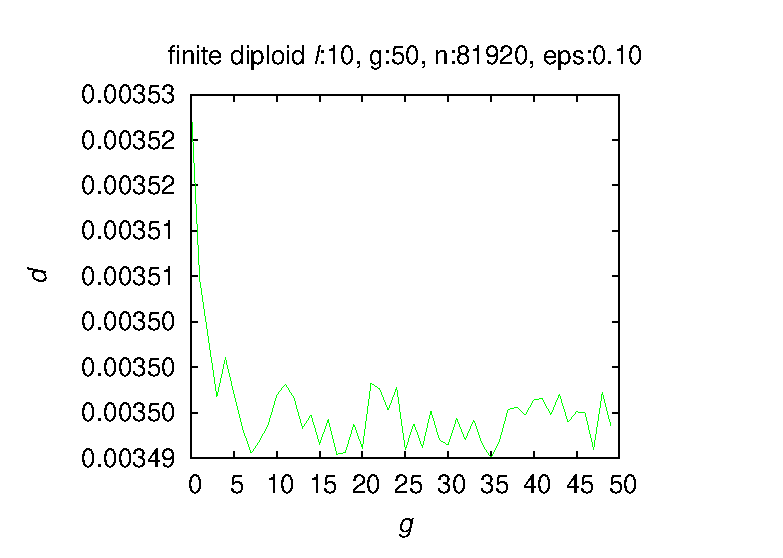
\includegraphics{figures/eps/vio/mu/b10/e0.1/n00081920_fin_dip.eps}}}\hspace{-3em}%
\subfloat{
\resizebox{8cm}{4.5cm}{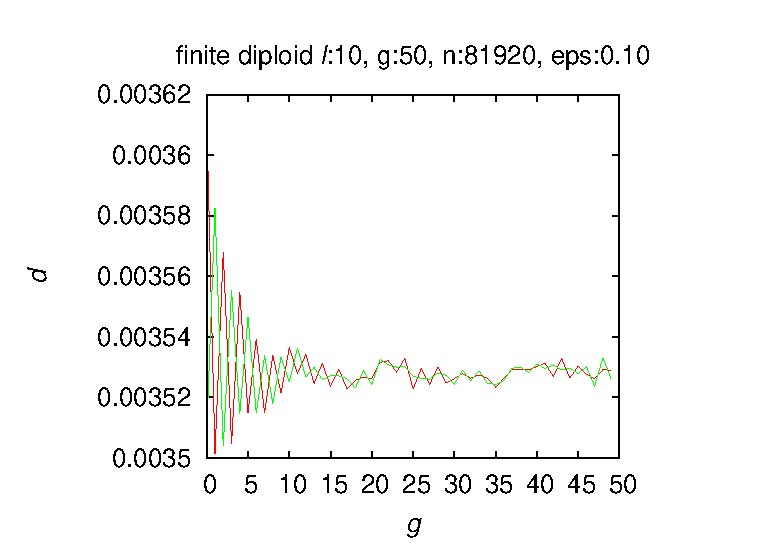
\includegraphics{figures/eps/vio/mu/b10/e0.1/n00081920_fin_dip_wovio.eps}}}\vspace{-1em}  \hspace{-3em}%
\end{center}

\begin{center}
\subfloat{
\resizebox{8cm}{4.5cm}{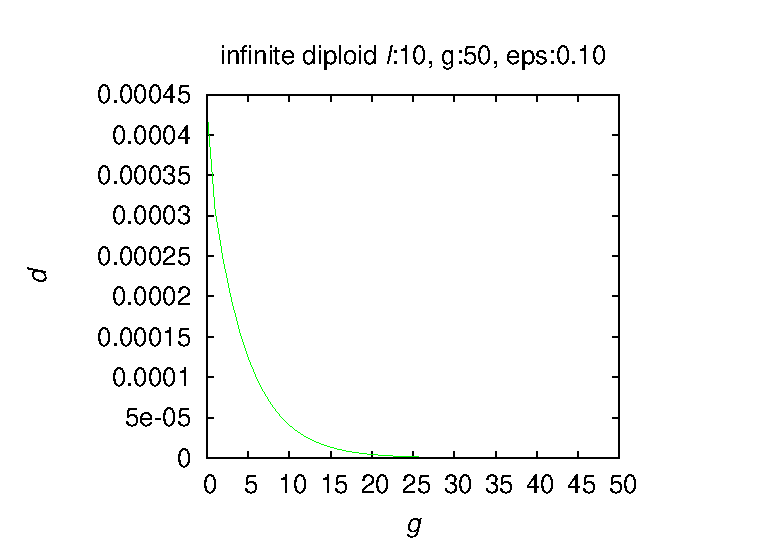
\includegraphics{figures/eps/vio/mu/b10/e0.1/inf_dip.eps}}}\hspace{-3em}%
\subfloat{
\resizebox{8cm}{4.5cm}{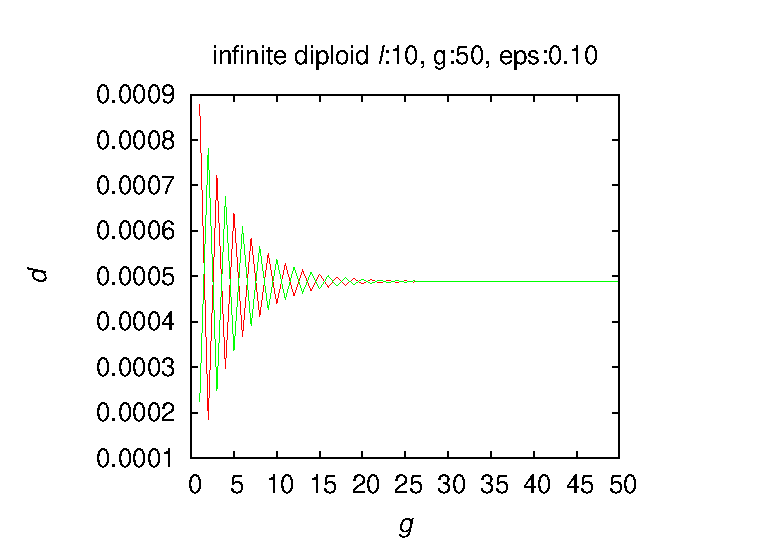
\includegraphics{figures/eps/vio/mu/b10/e0.1/inf_dip_wovio.eps}}}\vspace{-0.5em}  \hspace{-3em}%


\caption[\textbf{Infinite and finite diploid population behavior for $\bm{\mu}$ violation, genome length $\ell = 10$ and $\bm{\epsilon} = 0.1$}]{\textbf{Infinite and finite diploid population behavior for $\bm{\mu}$ violation, genome length $\ell = 10$ and $\bm{\epsilon} = 0.1$:} 
  In left column, $d'$ is distance of finite or infinite population to limit $\bm{z}^\ast$ for $g$ generations. In right column, $d$ is distance of finite or infinite population to limits $\bm{p}^\ast$ and $\bm{q}^\ast$. Green line is distance to $\bm{p*}$ and red line is distance to $\bm{q*}$.}
\label{oscillation_10d_vio_mu_0.1}
\end{center}
\end{figure}

% l = 12

\begin{figure}[h]
\begin{center}
\subfloat{
\resizebox{8cm}{4.5cm}{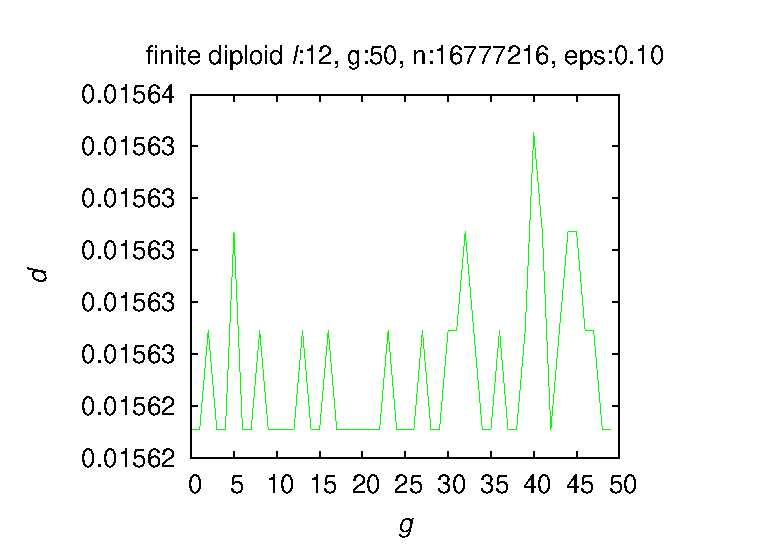
\includegraphics{figures/eps/vio/mu/b12/e0.1/n00004096_fin_dip.eps}}}\hspace{-3em}%
\subfloat{
\resizebox{8cm}{4.5cm}{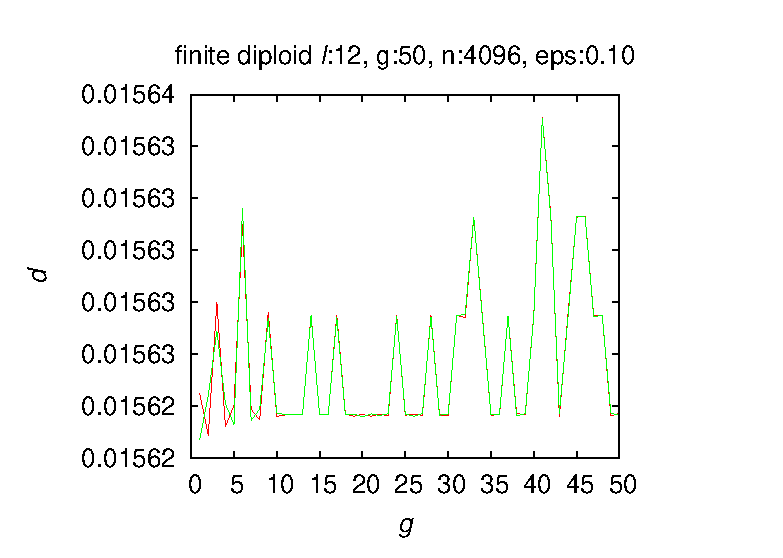
\includegraphics{figures/eps/vio/mu/b12/e0.1/n00004096_fin_dip_wovio.eps}}}\vspace{-1em}  \hspace{-3em}%
\end{center}
\begin{center}
\subfloat{
\resizebox{8cm}{4.5cm}{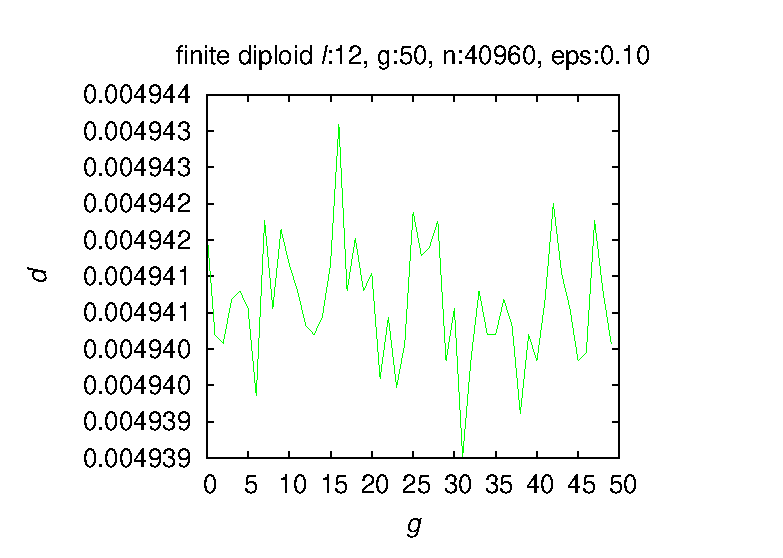
\includegraphics{figures/eps/vio/mu/b12/e0.1/n00040960_fin_dip.eps}}}\hspace{-3em}%
\subfloat{
\resizebox{8cm}{4.5cm}{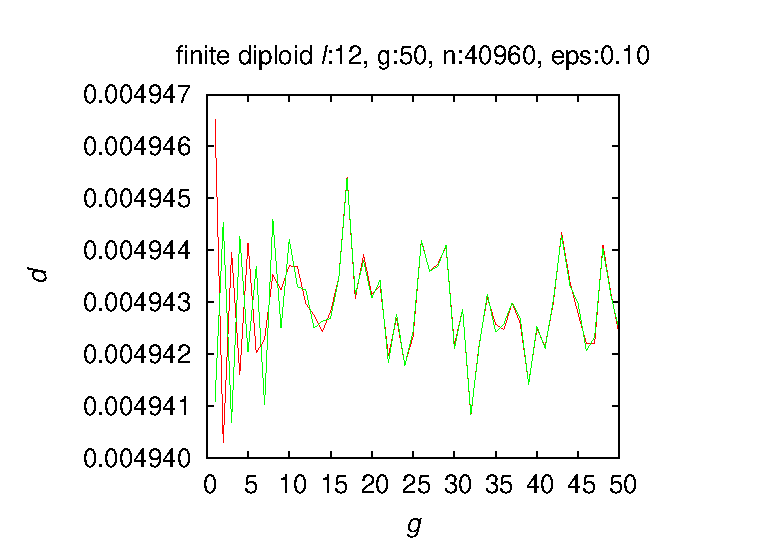
\includegraphics{figures/eps/vio/mu/b12/e0.1/n00040960_fin_dip_wovio.eps}}}\vspace{-1em}  \hspace{-3em}%
\end{center}


\begin{center}
\subfloat{
\resizebox{8cm}{4.5cm}{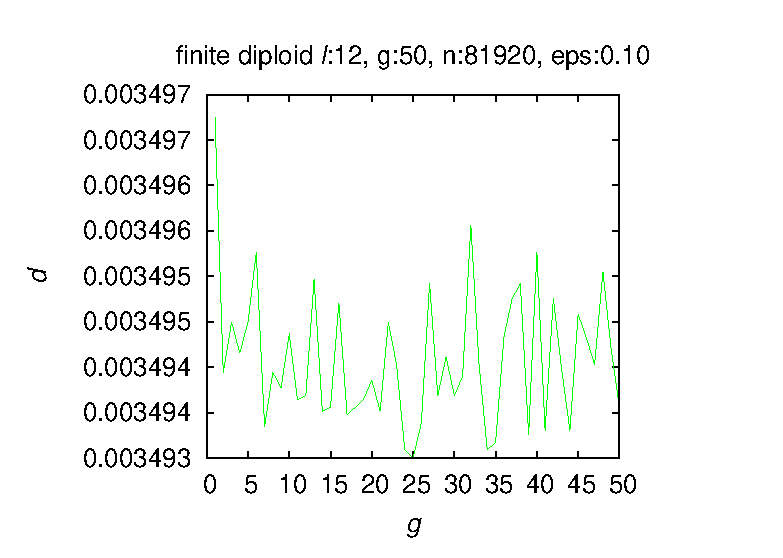
\includegraphics{figures/eps/vio/mu/b12/e0.1/n00081920_fin_dip.eps}}}\hspace{-3em}%
\subfloat{
\resizebox{8cm}{4.5cm}{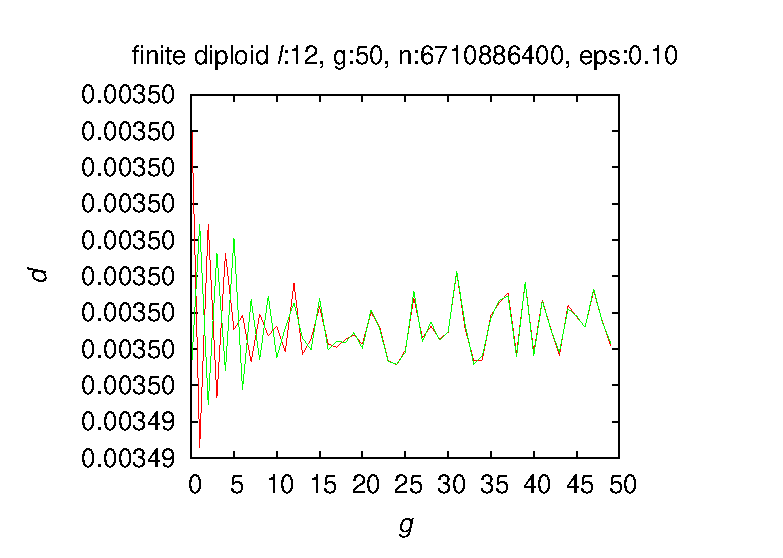
\includegraphics{figures/eps/vio/mu/b12/e0.1/n00081920_fin_dip_wovio.eps}}}\vspace{-1em}  \hspace{-3em}%
\end{center}

\begin{center}
\subfloat{
\resizebox{8cm}{4.5cm}{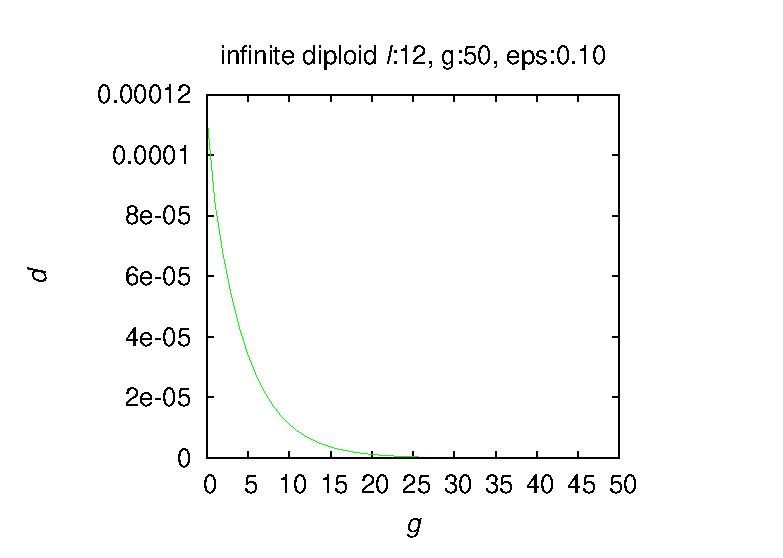
\includegraphics{figures/eps/vio/mu/b12/e0.1/inf_dip.eps}}}\hspace{-3em}%
\subfloat{
\resizebox{8cm}{4.5cm}{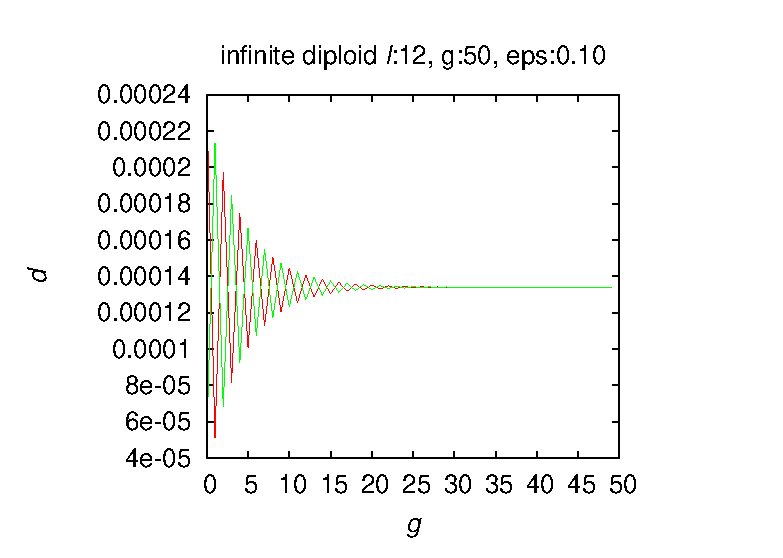
\includegraphics{figures/eps/vio/mu/b12/e0.1/inf_dip_wovio.eps}}}\vspace{-0.5em}  \hspace{-3em}%


\caption[\textbf{Infinite and finite diploid population behavior for $\bm{\mu}$ violation, genome length $\ell = 12$ and $\bm{\epsilon} = 0.1$}]{\textbf{Infinite and finite diploid population behavior for $\bm{\mu}$ violation, genome length $\ell = 12$ and $\bm{\epsilon} = 0.1$:} 
  In left column, $d'$ is distance of finite or infinite population to limit $\bm{z}^\ast$ for $g$ generations. In right column, $d$ is distance of finite or infinite population to limits $\bm{p}^\ast$ and $\bm{q}^\ast$. Green line is distance to $\bm{p*}$ and red line is distance to $\bm{q*}$.}
\label{oscillation_12d_vio_mu_0.1}
\end{center}
\end{figure}

% l = 14

\begin{figure}[h]
\begin{center}
\subfloat{
\resizebox{8cm}{4.5cm}{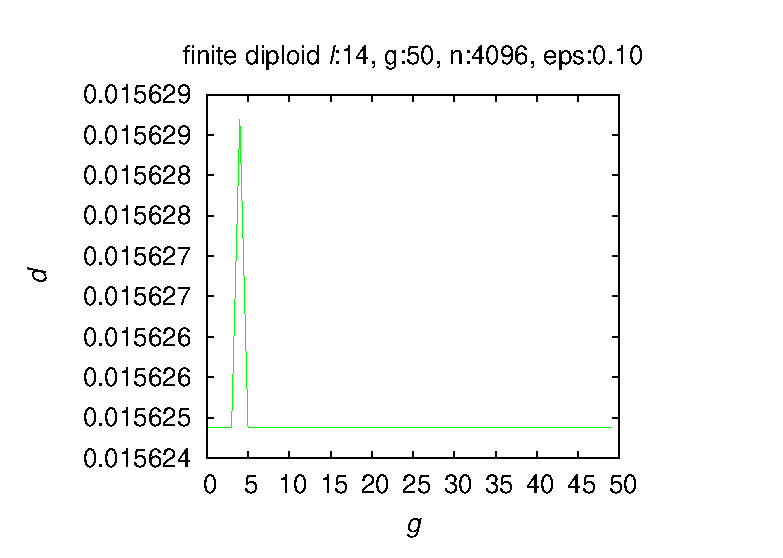
\includegraphics{figures/eps/vio/mu/b14/e0.1/n00004096_fin_dip.eps}}}\hspace{-3em}%
\subfloat{
\resizebox{8cm}{4.5cm}{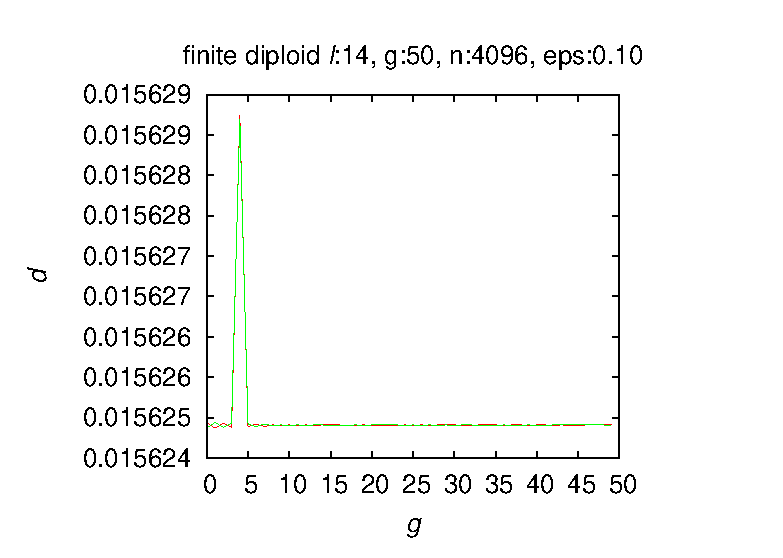
\includegraphics{figures/eps/vio/mu/b14/e0.1/n00004096_fin_dip_wovio.eps}}}\vspace{-1em}  \hspace{-3em}%
\end{center}
\begin{center}
\subfloat{
\resizebox{8cm}{4.5cm}{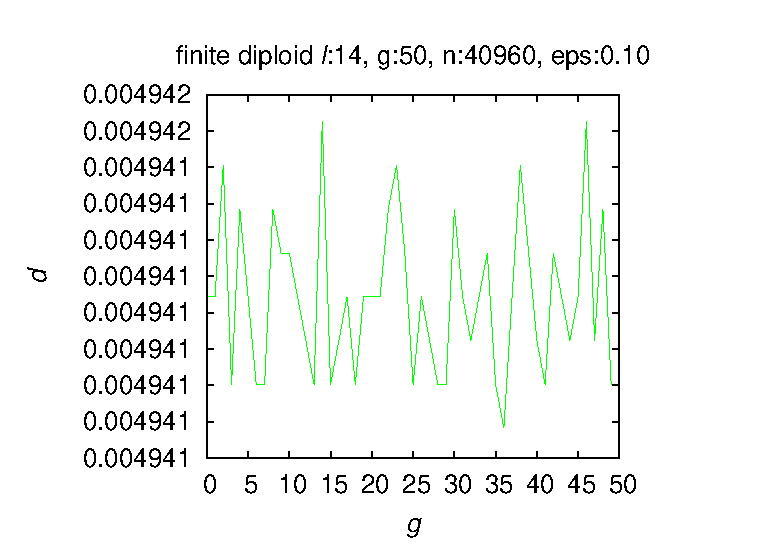
\includegraphics{figures/eps/vio/mu/b14/e0.1/n00040960_fin_dip.eps}}}\hspace{-3em}%
\subfloat{
\resizebox{8cm}{4.5cm}{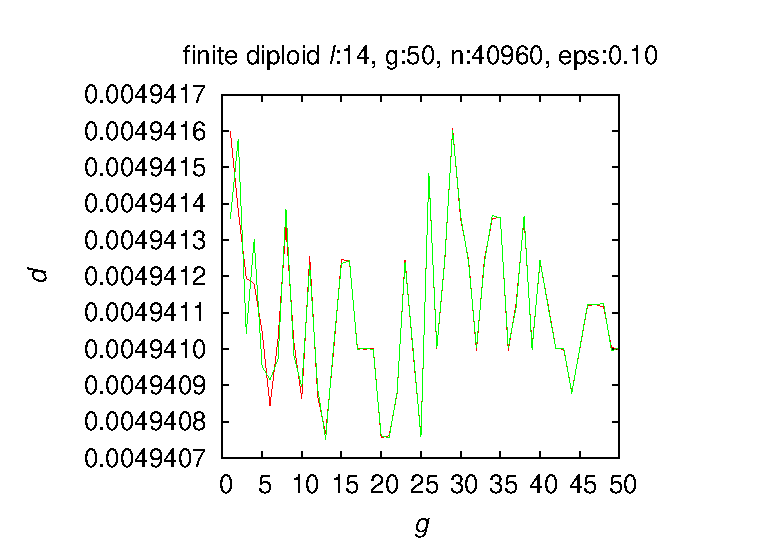
\includegraphics{figures/eps/vio/mu/b14/e0.1/n00040960_fin_dip_wovio.eps}}}\vspace{-1em}  \hspace{-3em}%
\end{center}


\begin{center}
\subfloat{
\resizebox{8cm}{4.5cm}{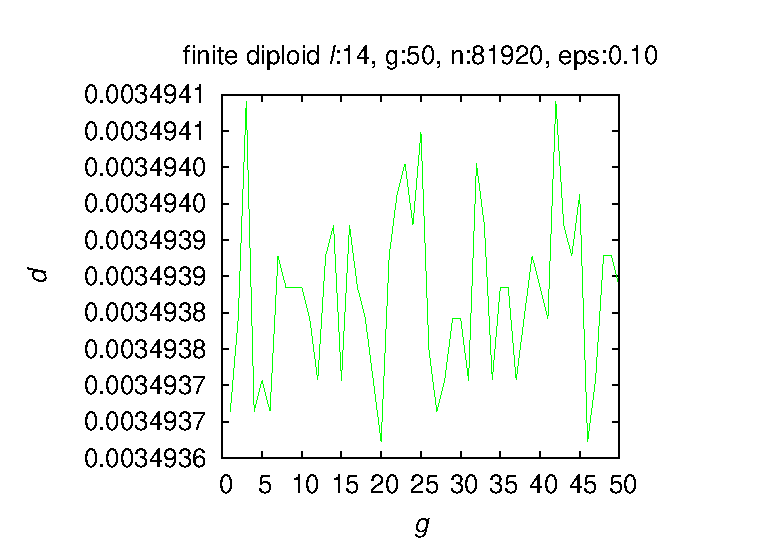
\includegraphics{figures/eps/vio/mu/b14/e0.1/n00081920_fin_dip.eps}}}\hspace{-3em}%
\subfloat{
\resizebox{8cm}{4.5cm}{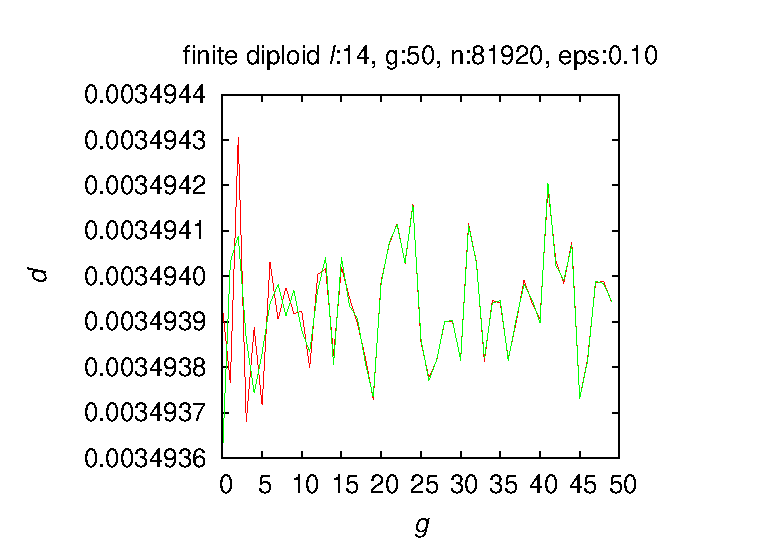
\includegraphics{figures/eps/vio/mu/b14/e0.1/n00081920_fin_dip_wovio.eps}}}\vspace{-1em}  \hspace{-3em}%
\end{center}

\begin{center}
\subfloat{
\resizebox{8cm}{4.5cm}{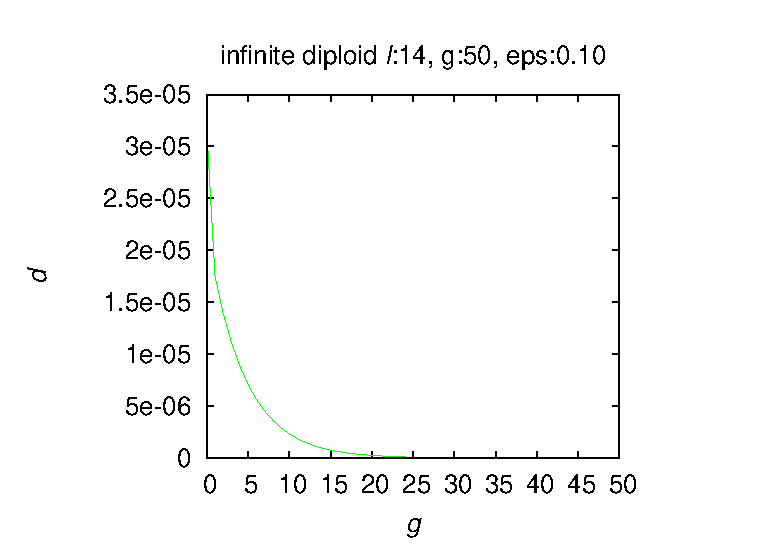
\includegraphics{figures/eps/vio/mu/b14/e0.1/inf_dip.eps}}}\hspace{-3em}%
\subfloat{
\resizebox{8cm}{4.5cm}{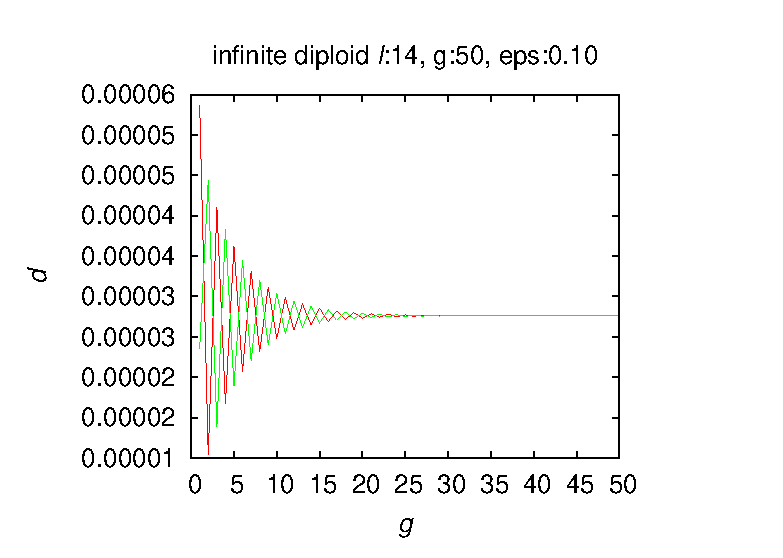
\includegraphics{figures/eps/vio/mu/b14/e0.1/inf_dip_wovio.eps}}}\vspace{-0.5em}  \hspace{-3em}%


\caption[\textbf{Infinite and finite diploid population behavior for $\bm{\mu}$ violation, genome length $\ell = 14$ and $\bm{\epsilon} = 0.1$}]{\textbf{Infinite and finite diploid population behavior for $\bm{\mu}$ violation, genome length $\ell = 14$ and $\bm{\epsilon} = 0.1$:} 
  In left column, $d'$ is distance of finite or infinite population to limit $\bm{z}^\ast$ for $g$ generations. In right column, $d$ is distance of finite or infinite population to limits $\bm{p}^\ast$ and $\bm{q}^\ast$. Green line is distance to $\bm{p*}$ and red line is distance to $\bm{q*}$.}
\label{oscillation_14d_vio_mu_0.1}
\end{center}
\end{figure}

% \clearpage
The right column in figures \ref{oscillation_8d_vio_mu_0.1} through \ref{oscillation_14d_vio_mu_0.1} 
shows distance of finite and infinite diploid populations to non-violation limits $\bm{p^\ast}$ and $\bm{q^\ast}$ with $\bm{\epsilon} \;=\; 0.1$. 
Those graphs indicate oscillating behavior of diploid population given violation. 
Both finite and infinite populations oscillate, and oscillation amplitudes decreases with time. 
Like in the haploid case, for $\bm{\epsilon} \;=\; 0.1$, oscillations in infinite populations die out quickly, 
but finite population oscillation does not. Rate of damping of ripples with $\bm{\epsilon} \;=\; 0.1$ is  
larger than with $\bm{\epsilon} \;=\; 0.01$. The all zeros mask created in mutation distribution with $\bm{\epsilon} \;=\; 0.1$ 
has a larger probability of being used during mutation as compared with the $\bm{\epsilon} = 0.01$ case.
More random wiggling of finite population is noticed than in case of $\bm{\epsilon} = 0.01$, and as value of $\ell$ 
increases, random wiggling is more prevalent.

The left column of figures \ref{oscillation_8d_vio_mu_0.1} through \ref{oscillation_14d_vio_mu_0.1} 
shows distance of finite and infinite diploid populations to limit $\bm{z^\ast}$ 
(limit with violation in mutation distribution $\bm{\mu}$) when $\bm{\epsilon} \;=\; 0.1$. 
The distance decreases as finite population size increases, 
and finite population shows behavior similar to infinite population behavior as population size grows. 
 
 \clearpage
 Average distance data for diploid population in case of violation in $\bm{\mu}$ distribution 
with $\bm{\epsilon} \;=\; 0.1$ are tabulated in table \ref{distanceMuDipEps0.1}. 
\begin{table}[ht]
\caption[\textbf{Distance measured for violation in $\bm{\mu}$ with $\bm{\epsilon} \;=\; 0.1$ for diploids}]{\textbf{Distance measured for violation in $\bm{\mu}$ with $\bm{\epsilon} \;=\; 0.1$ for diploids:} $\ell$ is genome length, 
average distance between finite and infinite population is tabulated in the last three columns, and last row is expected single step distance.}
\centering
\begin{tabularx}{0.75\textwidth}{ c *{3}{X}}
\toprule
$\ell$ & $N = 4096$ & $N = 40960$ & $N = 81920$ \\
\midrule
8 & 0.0156	&  0.0049	& 0.0035 \\
10 & 0.0156	&  0.0049	& 0.0035 \\
12 & 0.0156	&  0.0049	& 0.0035 \\
14 & 0.0156	&  0.0049	& 0.0035 \\
\midrule
$1/\sqrt{N}$ & 0.0156 & 0.0049 & 0.0035 \\
\bottomrule
\end{tabularx}
\label{distanceMuDipEps0.1}
\end{table}

Table \ref{distanceMuDipEps0.1} shows the average distance 
between finite population and infinite population agrees with the expected single step distance 
$1/\sqrt{N}$. 
 